% !TeX root = Bericht.tex
% !TeX spellcheck = de_DE

\section{Standpunkt 1965}
Der Bereich der Radioastronomie ist in den 30er aufgekommen und hat Astronomen §§ geöffnet. Während optische Lichtwellen leicht abgeschirmt werden (durch Staub und Gas), können Radiowellen aufgrund ihrer große Wellenlänge (und niedriger Energie) sich viel weiter fortpflanzen ohne starke Verluste zu erleiden. Deshalb können mit Radioteleskopen Objekte beobachtet werden, die große Entfernungen besitzen, s

Mitte der 60er Jahre wurde eine neue Klasse an astronomischen Objekten entdeckt. Im Optischen erscheinen diese entweder gar nicht oder nur sehr schwach und punktförmig, wie Sterne. Im Radiobereich, der in dem Jahrzehnt neu aufgeschlossen wurde, strahlen sie sehr stark und man erkennt zum Teil räumliche Ausdehnungen. Hinzu  kommt, dass das Spektrum das eines schwarzen Strahlers gar nicht ähnelt und Spektralinien zu sehen sind, die hohe Rotverschiebungen und somit hohe Enfernungen andeuten. Diese Objekte wurden aufgrund ihrer optischen Ähnlichkeit mit Sternen quasi-stellare-Objekte, kurz QSO oder Quasare, getauft. 

Was Quasare zu einzigartigen (und physikalisch äußerst problematischen) Objekten macht, sind folgende drei Beobachtungen:
\begin{enumerate}
	\renewcommand{\labelenumi}{\arabic{enumi})}
	\item Falls die Rotverschiebung der Spektrallinien (\( z > 0.1\)) der Expansion des Universums zugeschrieben werden kann, dann haben Quasare Entfernungen von über \( 500 \unit{Mpc} \).
	\item Der gemessene Fluss von Quasaren ist hoch.
	\item Der Strahlungsfluss von Quasaren verfielfacht sich innerhalb von Tagen.
\end{enumerate}

Stimmen diese drei Aussagen/Beobachtungen, dann haben wir es bei Quasaren mit Objekten zu tun, deren Kernregion die Größe des Sonnensystems hat (Aussage 3), ein vielfaches der Milchstraße strahlt (Aussage 1 \& 2). 

Der gemessene Fluss kann unter der Annahme von Isotropie 
Die größe kernregion

 


\begin{figure}[H]
	\centering
	\begin{subfigure}{.45\textwidth}
		\centering
		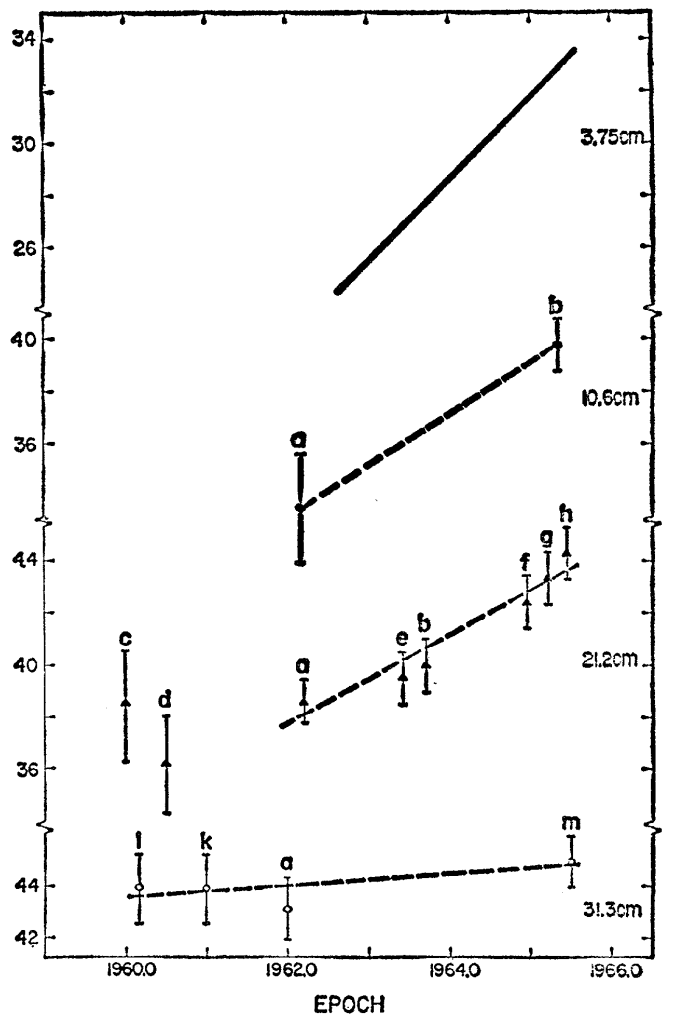
\includegraphics[width=\linewidth]{oldflux}
	\end{subfigure}%
	\begin{subfigure}{.55\textwidth}
		\centering
		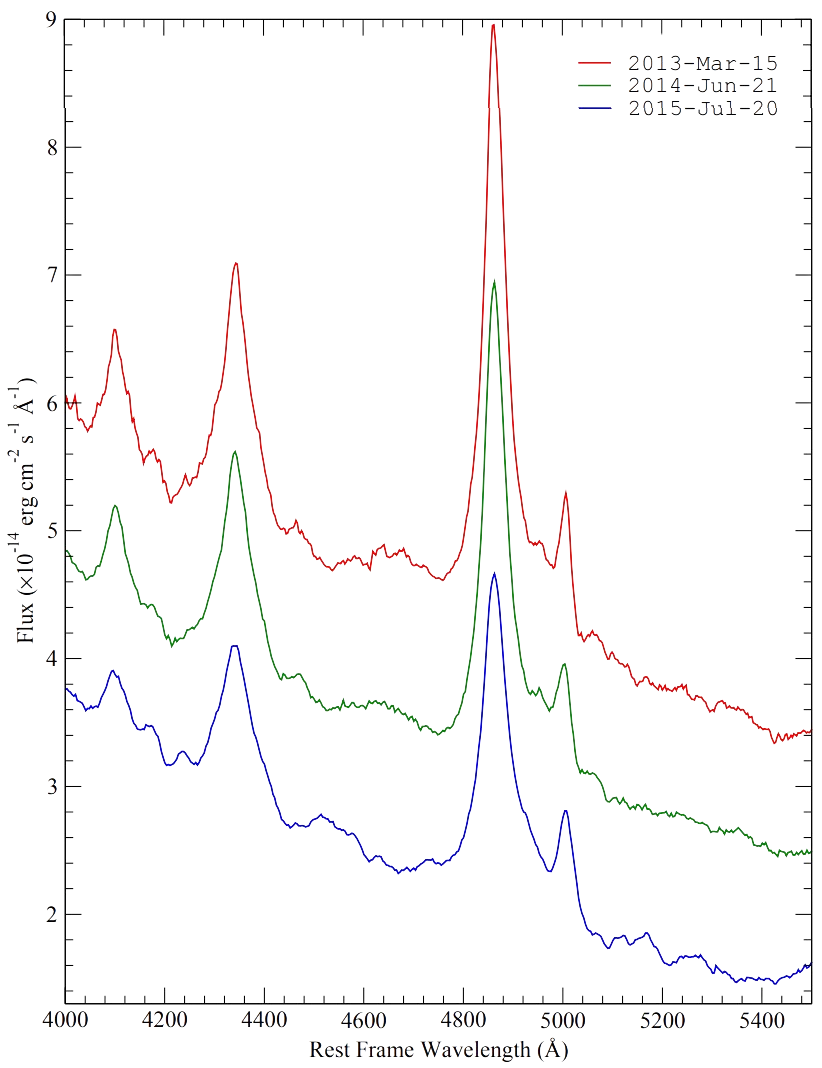
\includegraphics[width=\linewidth]{newflux}
	\end{subfigure}
	\caption{Links ist der gemessene Fluss auf die Zeit aufgetragen. An Beobachtungen die bei gleichen Wellenlängen durchgeführt wurden, sind Geraden angepasst worden. In der rechten Abbildung ist der gemessene Fluss des gleichen Quasars auf die Wellenlänge für drei Verschiedene Messreihen (farblich hervorgehoben) aufgetragen.}
	\label{fig:quasarflux}
\end{figure}

In \autoref{fig:quasarflux} sind 
In der Linken Abbildung aus 1965 \autocite{oldflux} sind Flussmessungen bei verschiednen Wellenlängen zu unterschiedlichen Zeitpunkten angegeben. Die gemessene Flussdichte ist mit Fehlerbalken auf den Beobachtungszeitpunkt aufgetragen, die Unterscheidung der Spektralbänder entsteht automatisch durch den Unterschied der Flüsse bei unterschiedlichen Wellenlängen. Auf Messungen aus dem gleichen Spektralband wurden lineare Regressionen angewendet und die erhaltenen Geraden sind strichliert dargestellt. 

In der rechten Abbildung aus 2020 \autocite{newflux} ist die Flussdichte auf die Wellenlänge aufgetragen, wobei drei farblich unterscheidbare Kurven drei Messungen aus 2013 bis 2015, mit jeweils einem Jahr Abstand, darstellen. 

Man erkennt, dass die Flussdichte im Zeitraum von 6 Jahren in allen Wellenlängen zugenommen hat. 

Drastische Helligkeitsschwankungen sind in der Astronomie nichts neues, das Problem ist die Kombination aus der Stärke und Geschwindigkeit der Fluktuationen. Damit sich ein ausgedehntes Objekt 
Wir haben es hier also mit 


Eine erhöhte Flussdichte kann man entweder durch einen erhöhten gesamten Energieausstoß oder durch eine vergrößerte Oberfläche, welche mit der gleichen Energiedichte strahlt. Prozesse, die so schnell den Energieausstoß auf den Größenordnungen wie es bei Quasaren beobachtet wird erhöht, sind schwer.

Eine vergrößerung der strahlenden Oberfläche kann zb durch Explosionen leicht gemacht werden, reicht aber aus klassischer Sicht nicht aus, um die Beobachtungen zu erklären. Betrachtet man dieses Argument aber relativistisch, sieht das ganze aber anders aus.

Betrachte eine Explosion, welche sich sphärisch vom Mittelpunkt \( S \) glaichförmig mit der Geschwindigkeit \( v \) ausbreitet. Im klassischen Regime \( v \ll c \) erscheint die sich ausbreitene Oberfläche für einen Beobachter \( O \) im Abstand \( R \ll vt \) kreisförmig (2D Projektion). Der Radius des Kreises nach der Zeit \( t \) (\( t \) wird ab dem Zeitpunkt gemessen, an dem die Explosion in \( O \) beobachtet wird) ist dabei \( r = vt \), und der Winkeldurchmesser beträgt \( \theta = 2\arctan(\tfrac{vt}{R}) \approx 2\tfrac{vt}{R} \).

Breitet sich die Explosion aber mit relativistischen Geschwindigkeiten aus \( v ~ c \) stimmt das klassische Bild nicht mehr. Aufgrund der Endlichkeit der Lichtgeschwindigkeit, wird in \( O \) kein "Snapshot" der Explosion beobachtet, das Licht, welches Gleichzeitig eintrifft und somit das gesehen Bild erzeugt, wurde an unterschiedlichen Orten der Explosion zu verschiedenen Zeiten losgeschickt. Die Expansion erscheint also nicht mehr perfekt sphärisch, sondern wie ein Ellipsoid (siehe autoref). 





